\documentclass{article}

\usepackage{siunitx} % Provides the \SI{}{} and \si{} command for typesetting SI units
\usepackage{graphicx} % Required for the inclusion of images
\usepackage{amsmath} % Required for some math elements 
\usepackage[export]{adjustbox} % loads also graphicx
\usepackage{listings}
\usepackage{matlab-prettifier}
\usepackage{float}
\usepackage[most]{tcolorbox}
\usepackage{amsfonts}
\usepackage{color}
\usepackage{titlesec}
\usepackage{caption}
\usepackage{subcaption}

\newcommand{\R}{\mathbb{R}}

\usepackage{xcolor}

\DeclareCaptionFont{white}{\color{white}}
\DeclareCaptionFormat{listing}{%
  \parbox{\textwidth}{\colorbox{gray}{\parbox{\textwidth}{#1#2#3}}\vskip-4pt}}
\captionsetup[lstlisting]{format=listing,labelfont=white,textfont=white}
\lstset{frame=lrb,xleftmargin=\fboxsep,xrightmargin=-\fboxsep}
\titleformat{\section}[runin]
  {\normalfont\Large\bfseries}{\thesection}{1em}{}
\titleformat{\subsection}[runin]
  {\normalfont\large\bfseries}{\thesubsection}{1em}{}


\setlength\parindent{0pt} % Removes all indentation from paragraphs

\renewcommand{\labelenumi}{\alph{enumi}.} % Make numbering in the enumerate environment by letter rather than number (e.g. section 6)

%\usepackage{times} % Uncomment to use the Times New Roman font

%----------------------------------------------------------------------------------------
%	DOCUMENT INFORMATION
%----------------------------------------------------------------------------------------

\title{AMATH 353: Homework 12 \\Due May, 18 2018 \\ ID: 1064712} % Title

\author{Trent \textsc{Yarosevich}} % Author name

\date{\today} % Date for the report

\begin{document}
\maketitle % Insert the title, author and date
\setlength\parindent{1cm}

\begin{center}
\begin{tabular}{l r}
%Date Performed: December 1, 2017 \\ % Date the experiment was performed
Instructor: Jeremy Upsal % Instructor/supervisor
\end{tabular}
\end{center}

% If you wish to include an abstract, uncomment the lines below
% \begin{abstract}
% Abstract text
% \end{abstract}

%----------------------------------------------------------------------------------------
%	SECTION 1
%----------------------------------------------------------------------------------------
\section*{Part 1}
\subsection*{a.)}
Because the PDE in question is homogeneous, we have $x = c(u_o(x_0))t + x_0$. For this equation, $c(u(x,t)) = u(x, t)$. From this we get the following:
\begin{equation}
\begin{aligned}
u(x,0) = u_0(x_0) = e^{-x^2}\\
\frac{du}{dt} = 0\\
u(x(t), t) = A = e^{-x_0^2}
\end{aligned}
\end{equation}
And the characteristic lines:
\begin{tcolorbox}[minipage,colback=white,arc=0pt,outer arc=0pt]
\begin{equation}
\begin{aligned}
x = x_0 + te^{-x^2}\\
t = (x - x_0)e^{x^2}
\end{aligned}
\end{equation}
\end{tcolorbox}
\subsection*{b.)}
\begin{figure}[H]
  \centering
    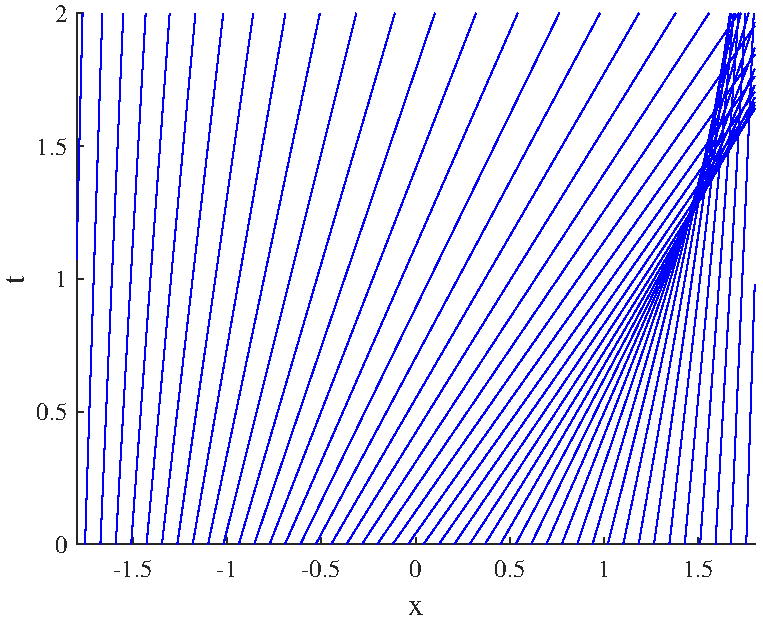
\includegraphics[width=\textwidth]{hw_13_plot1.pdf}
    \caption{$x_0 \in [-1.8, 1.8]$}
\end{figure}
\subsection*{c.)}
I wrote a script in matlab to find the roots for $f(x_0) = x_0 - x + te^{-x^2}$, which is included in my HW submission.
\subsection*{d.) and e.)}
Below are the plots, using $x_0$ values from my rootfinder, for $t = 0, 0.6, 0.9, 1.18$ and $x \in [-1.8, 1.8]$ with a mesh of values. From the first figure, it is clear that at $t=0$ the rootfinder is returning the correct values, yielding the profile of $u_0(x_0) = e^{-x^2}$. As the figures below show, as $t$ increases, the top of the profile has a faster rate of change than the bottom, causeing a 'crashing wave' to form. This is to be expected, since the time velocity of the PDE is depending on both the spatial velocity and the value of $u$ itself, thus the larger $u$ values have larger time velocity.
\begin{figure}[H]
  \centering
  \begin{minipage}[b]{0.49\textwidth}
    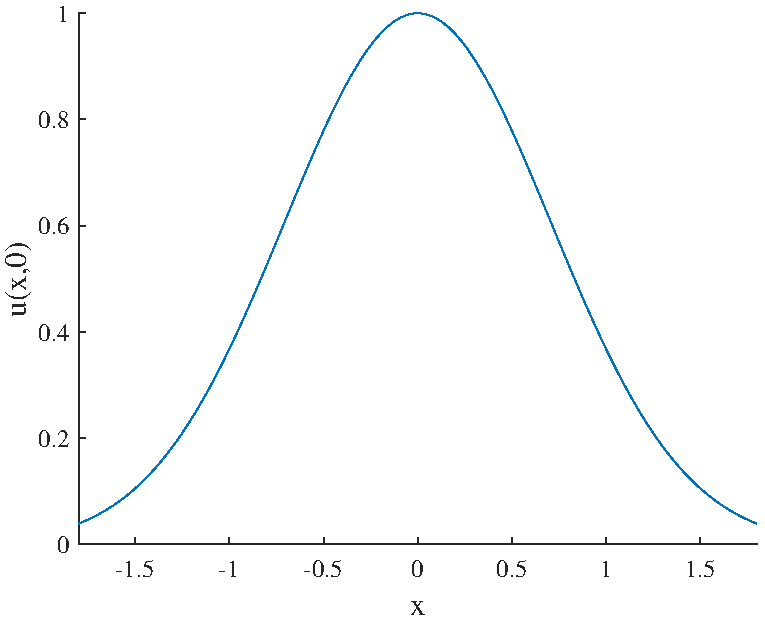
\includegraphics[width=\textwidth]{hw_13_plot2.pdf}
    \caption{$t = 0$}

  \end{minipage}
  \hfill
  \begin{minipage}[b]{0.49\textwidth}
    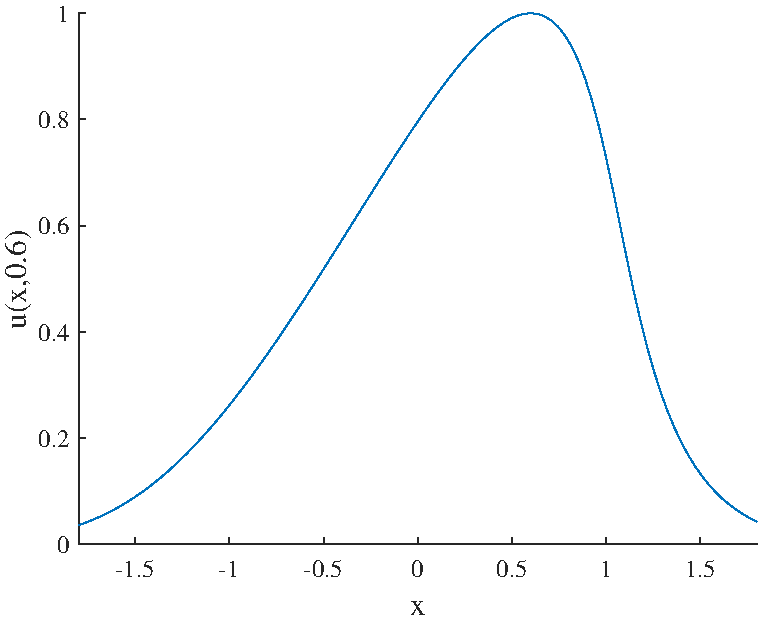
\includegraphics[width=\textwidth]{hw_13_plot3.pdf}
    \caption{$t = 0.6$}

  \end{minipage}
    \hfill
  \begin{minipage}[b]{0.49\textwidth}
    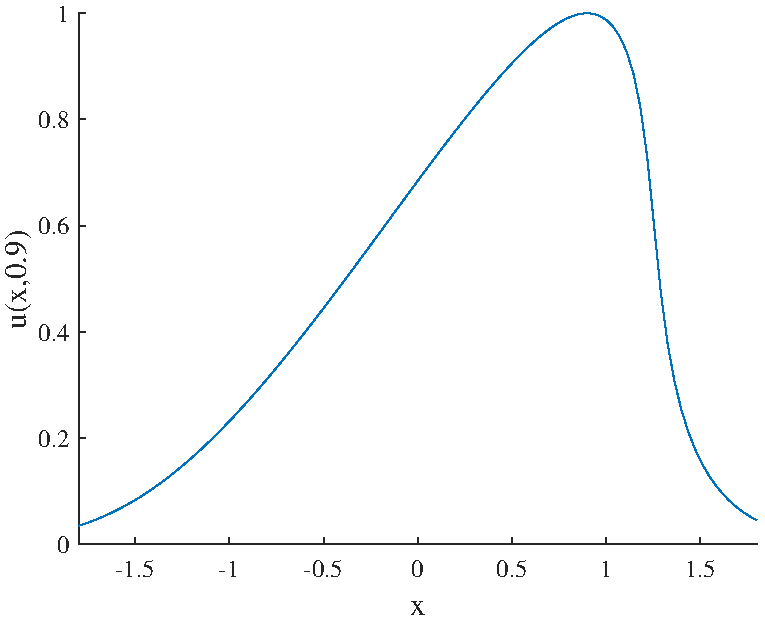
\includegraphics[width=\textwidth]{hw_13_plot4.pdf}
    \caption{$t = 0.9$}

  \end{minipage}
    \hfill
  \begin{minipage}[b]{0.49\textwidth}
    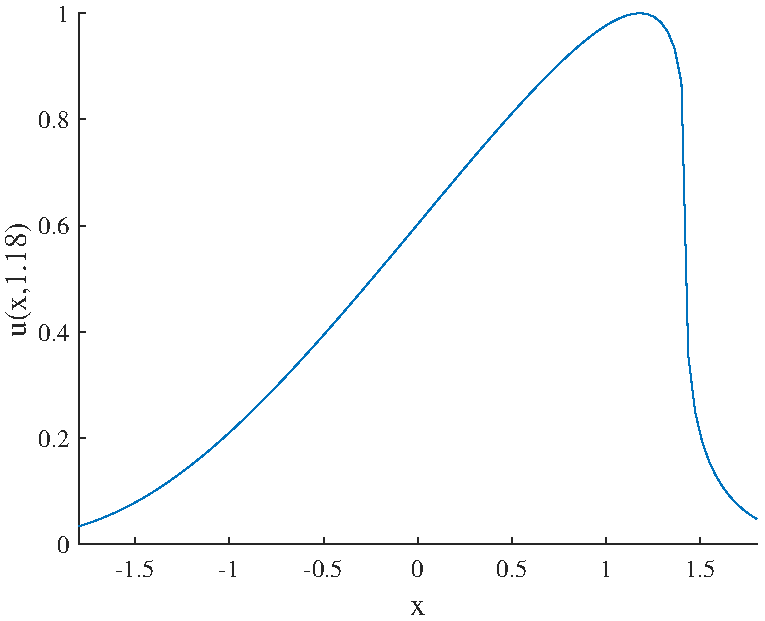
\includegraphics[width=\textwidth]{hw_13_plot5.pdf}
    \caption{$t = 1.18$}

  \end{minipage}
\end{figure}
\subsection*{f.)}
When my rootfinder is used to plot the values at $t=1.5$, it appears to get 'stuck' at the point of the wave crashing and falling over. This occurs at the point that the characteristics start to cross, which by closely examining (zooming in) on Figure 1, would seem to happen around $t = 1.2$. Below are two plots using my rootfinder, of $t = 1.5$ and $t = 2.5$. In both, we see an abrupt change in the value of $u$, caused by crossing characteristic lines which result in the value of $u$ 'jumping' between two $x_0$ values produced by my rootfinder. The plot at $t=2.5$ shows what the profile looks like as even more $x_0$ values fall inside the range where they begin to cross.

\begin{figure}[H]
  \centering
  \begin{minipage}[b]{0.49\textwidth}
    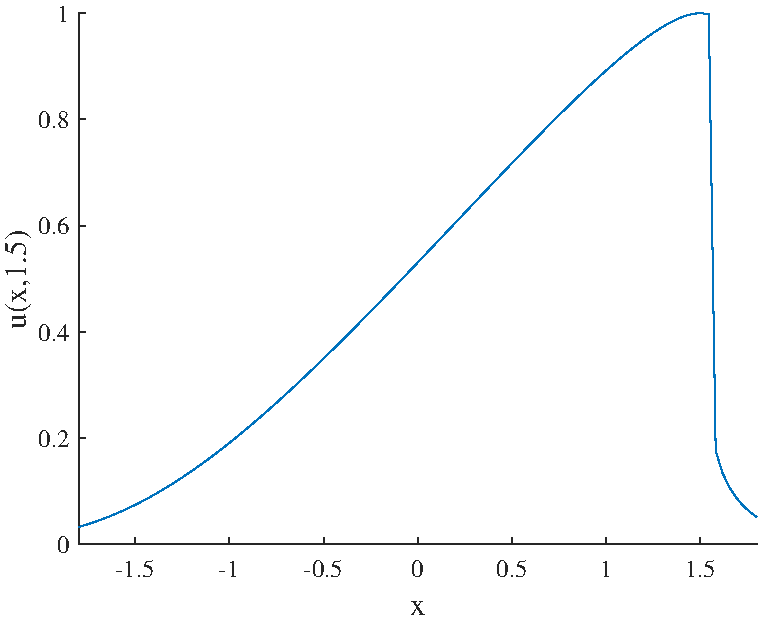
\includegraphics[width=\textwidth]{hw_13_plot6.pdf}
    \caption{$t = 1.5$}

  \end{minipage}
  \hfill
  \begin{minipage}[b]{0.49\textwidth}
    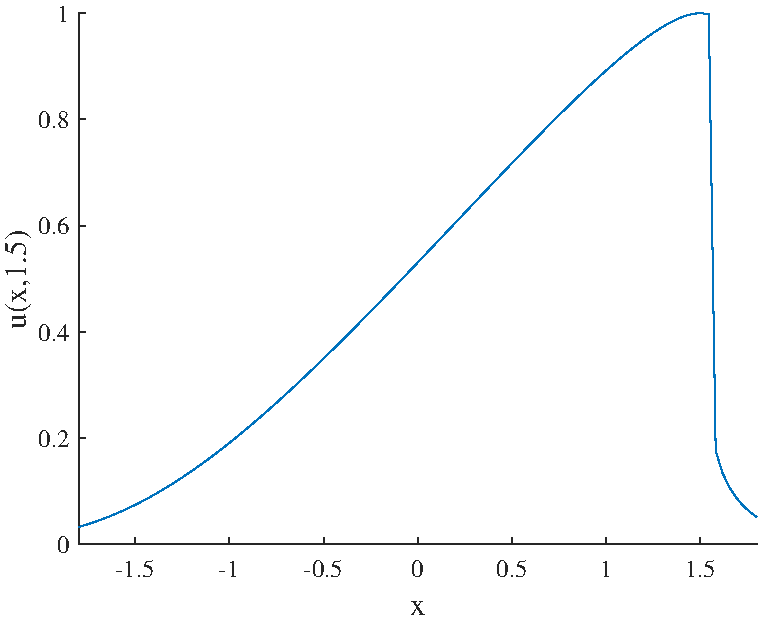
\includegraphics[width=\textwidth]{hw_13_plot6.pdf}
    \caption{$t = 2.5$}

  \end{minipage}
    \hfill
\end{figure}
\section*{Part 2}
\subsection*{a.)}
Given the provided initial condition, and the fact that the PDE is homogeneous, we have the following:
\begin{equation}
\begin{aligned}
u(x(t), t) = u(x(0), 0) = u_0(x_0) = \frac{1}{1+x_0^2}\\
\frac{du}{dt} = 0\\
u(x(t), t) = A = \frac{1}{1+x_0^2}
\end{aligned}
\end{equation}
And then for the characteristic lines:
\begin{equation}
\begin{aligned}
c(u(x,t)) = u(x,t)^2\\
u(x,t)^2 = u_0(x_0)^2 = \frac{1}{(1+x_0^2)^2}
\end{aligned}
\end{equation}
We then plug this into the formula $x = x_0 + tc(u(x,t))$ to arrive at the equation for the characteristics:
\begin{tcolorbox}[minipage,colback=white,arc=0pt,outer arc=0pt]
\begin{equation}
x = x_0 + \frac{t}{(1+x_0^2)^2}
\end{equation}
\end{tcolorbox}
Here is a plot of these characteristic curves:
\begin{figure}[H]
  \centering
    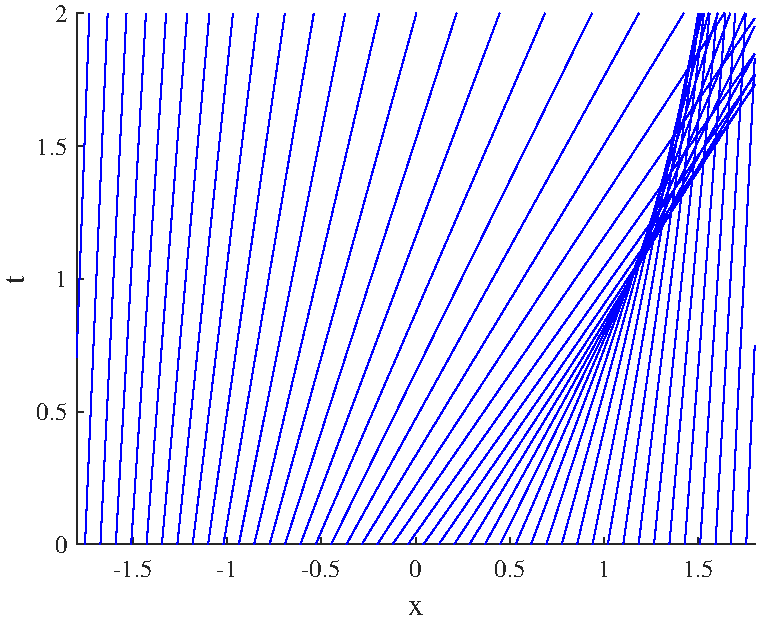
\includegraphics[width=\textwidth]{hw_13_plot8.pdf}
    \caption{$x_0 \in [-2, 2]$}
\end{figure}
\subsection*{(c) - (d)}
First, we need to take the implicit derivative of equation (5) above in order to find $\frac{dx_0}{dx}$, so that we can examine at what point in time it blows up to $\infty$:
\begin{equation}
\begin{aligned}
\frac{d}{dx}x = \frac{d}{dx} \Big[x_0 + \frac{t}{(1+x_0^2)^2}\Big]\\
1 = \frac{dx_0}{dx} + t\frac{d}{dx}\Big[(1+x_0^2)^{-2}\Big]\\
1 = \frac{dx_0}{dx} + t\Big[t(-2(1 + x_0^2)^{-3}(2x_0)(\frac{dx_0}{dx})\Big]\\
1 = \frac{dx_0}{dx}\Big[\frac{-4tx_0}{(1+x_0^2)^3}\Big]
\end{aligned}
\end{equation}
\begin{tcolorbox}[minipage,colback=white,arc=0pt,outer arc=0pt]
\begin{equation}
\frac{dx_0}{dx} = \frac{1}{\frac{-4tx_0}{(1+x_0^2)^3} + 1}
\end{equation}
\end{tcolorbox}
Examining this equation, it is clear that it can only go to $\infty$ when the denominator approaches zero, and so we have:
\begin{equation}
\begin{aligned}
\frac{-4tx_0}{(1+x_0^2)^3} + 1 = 0\\
t = \frac{(1+x_0^2)^3}{4x_0}
\end{aligned}
\end{equation}
We are interested in the lowest time $t$ at which this equation holds, so we will use this last equation to make a function of $x_0$, take the derivative of that function, and see at what $x_0$ it is equal to zero.
\end{document}